\section{Decomposi\c{c}\~ao via Programa\c{c}\~ao Din\^amica Dual Estoc\'astica}
\label{sec:pdde}

A Programa\c{c}\~ao Din\^amica Dual Estoc\'astica (PDDE) foi introduzida por \citeonline{pereira1991} como m\'etodo de decomposi\c{c}\~ao para problemas de programa\c{c}\~ao estoc\'astica multiestágio de grande porte. A ideia central \'e evitar a constru\c{c}\~ao expl\'icita de toda a \'arvore de cen\'arios em mem\'oria, substituindo-a por uma estrutura recursiva baseada em subproblemas por est\'agio e aproxima\c{c}\~oes lineares por partes das fun\c{c}\~oes de valor futuro.

\subsection{Representa\c{c}\~ao por Grafo de Pol\'itica}
\label{subsec:policy_graph}

A PDDE opera sobre um \emph{grafo de pol\'itica} (\textit{policy graph}) \cite{dowson2021}, uma representa\c{c}\~ao do problema como um grafo dirigido ac\'iclico em que cada n\'o corresponde a um subproblema de est\'agio. Diferentemente da DEQ, que mant\'em em mem\'oria toda a \'arvore de cen\'arios --- com uma c\'opia das vari\'aveis de decis\~ao para cada trajet\'oria completa, fazendo o problema crescer exponencialmente com o n\'umero de est\'agios e ramos ---, o grafo de pol\'itica resolve um subproblema compacto por n\'o e aproxima a fun\c{c}\~ao de valor futuro por cortes de Benders, de modo que o espa\c{c}o de decis\~ao em cada est\'agio \'e independente do tamanho total da \'arvore. Neste trabalho, cada m\^es $t$ do horizonte de planejamento \'e dividido em dois momentos distintos:

\begin{enumerate}
  \item \textbf{N\'o de decis\~ao} $(t, 0)$: a comercializadora escolhe os volumes de compra e venda $q_t = (q^B_t, q^S_t)$ com base apenas no estado herdado do est\'agio anterior. O cen\'ario do m\^es ainda n\~ao \'e conhecido.
  \item \textbf{N\'os de liquida\c{c}\~ao} $(t, c)$, um para cada cen\'ario $c$ do m\^es: ap\'os a decis\~ao, ocorre a transi\c{c}\~ao probabil\'istica para um dos n\'os de liquida\c{c}\~ao, onde se revelam o PLD e a gera\c{c}\~ao f\'isica e apura-se o resultado financeiro do est\'agio.
\end{enumerate}

Essa separa\c{c}\~ao entre o momento de decis\~ao e o momento de realiza\c{c}\~ao das incertezas incorpora naturalmente a n\~ao antecipatividade na pr\'opria estrutura do modelo, sem necessidade de restri\c{c}\~oes expl\'icitas como na formula\c{c}\~ao DEQ. A Figura~\ref{fig:policy_graph_pdde} ilustra essa estrutura para um horizonte de tr\^es meses com tr\^es cen\'arios por est\'agio.

\begin{figure}[H]
    \centering
    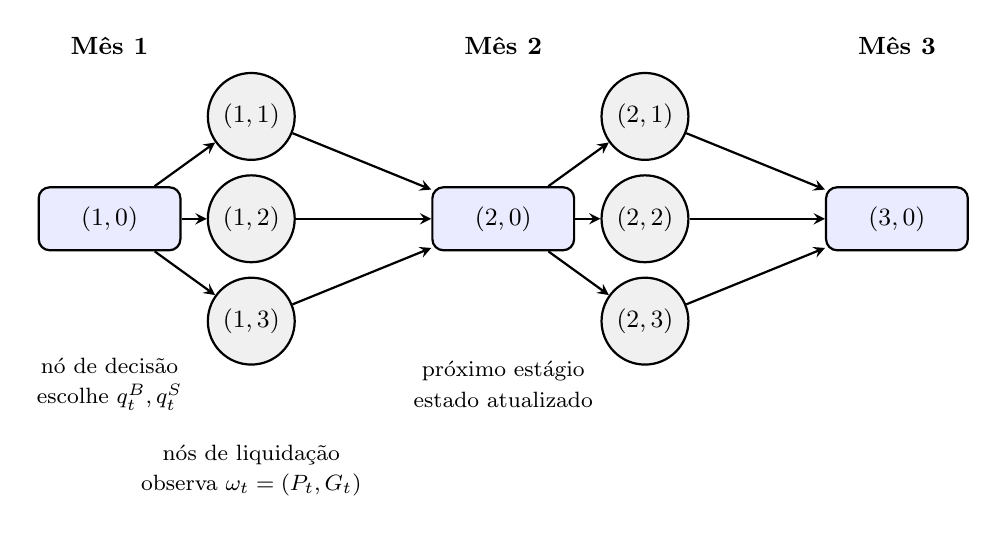
\begin{tikzpicture}[
        dec/.style={rectangle, rounded corners, draw=black, thick, minimum width=1.8cm, minimum height=0.8cm, fill=blue!8},
        scen/.style={circle, draw=black, thick, minimum size=0.8cm, fill=gray!12},
        edge/.style={->, thick, >=stealth},
        font=\small
    ]

    % Nós de decisão
    \node[dec] (d1) at (0,0) {$(1,0)$};
    \node[dec] (d2) at (5,0) {$(2,0)$};
    \node[dec] (d3) at (10,0) {$(3,0)$};

    % Cenários do mês 1
    \node[scen] (s11) at (1.8,1.3) {$(1,1)$};
    \node[scen] (s12) at (1.8,0) {$(1,2)$};
    \node[scen] (s13) at (1.8,-1.3) {$(1,3)$};

    % Cenários do mês 2
    \node[scen] (s21) at (6.8,1.3) {$(2,1)$};
    \node[scen] (s22) at (6.8,0) {$(2,2)$};
    \node[scen] (s23) at (6.8,-1.3) {$(2,3)$};

    % Setas mês 1
    \draw[edge] (d1) -- (s11);
    \draw[edge] (d1) -- (s12);
    \draw[edge] (d1) -- (s13);

    \draw[edge] (s11) -- (d2);
    \draw[edge] (s12) -- (d2);
    \draw[edge] (s13) -- (d2);

    % Setas mês 2
    \draw[edge] (d2) -- (s21);
    \draw[edge] (d2) -- (s22);
    \draw[edge] (d2) -- (s23);

    \draw[edge] (s21) -- (d3);
    \draw[edge] (s22) -- (d3);
    \draw[edge] (s23) -- (d3);

    % Legendas
    \node[align=center] at (0,-2.1) {\footnotesize n\'o de decis\~ao\\\footnotesize escolhe $q_t^B,q_t^S$};
    \node[align=center] at (1.8,-3.2) {\footnotesize n\'os de liquida\c{c}\~ao\\\footnotesize observa $\omega_t=(P_t,G_t)$};
    \node[align=center] at (5,-2.1) {\footnotesize pr\'oximo est\'agio\\\footnotesize estado atualizado};

    % Títulos dos estágios
    \node at (0,2.2) {\textbf{M\^es 1}};
    \node at (5,2.2) {\textbf{M\^es 2}};
    \node at (10,2.2) {\textbf{M\^es 3}};

    \end{tikzpicture}
    \caption{Estrutura do \textit{policy graph} utilizado na PDDE: em cada m\^es, a decis\~ao de contrata\c{c}\~ao \'e tomada antes da realiza\c{c}\~ao do cen\'ario, e a liquida\c{c}\~ao ocorre ap\'os a revela\c{c}\~ao das incertezas.}
    \label{fig:policy_graph_pdde}
    \vspace{-5mm}
\end{figure}

\subsection{Vetor de Estado e Equa\c{c}\~ao de Transi\c{c}\~ao}
\label{subsec:estado_transicao}

O estado da comercializadora no in\'icio do est\'agio $t$ \'e representado pelo vetor:
%
\begin{equation}
  y_t = (x_t,\; v_t,\; c_t),
  \label{eq:vetor_estado}
\end{equation}
%
onde $x_t$ \'e o saldo de caixa acumulado, $v_t$ re\'une as posi\c{c}\~oes f\'isicas l\'iquidas ainda ativas na carteira e $c_t$ re\'une os fluxos financeiros associados a esses contratos. As decis\~oes do est\'agio s\~ao os volumes de compra e venda $q_t = (q^B_t, q^S_t)$, definidos antes da realiza\c{c}\~ao das incertezas $\omega_t = (P_{s,t,\omega}, G_{s,t,\omega})_{s \in \mathcal{S}}$.

A din\^amica do sistema \'e descrita pela equa\c{c}\~ao de transi\c{c}\~ao de estados:
%
\begin{equation}
  y_{t+1} = T_t(y_t,\, q_t,\, \omega_t),
  \label{eq:transicao_estado}
\end{equation}
%
onde $T_t(\cdot)$ agrega as equa\c{c}\~oes de atualiza\c{c}\~ao da mem\'oria f\'isica da carteira, da mem\'oria financeira dos contratos vigentes e do saldo de caixa, de forma an\'aloga \`as equa\c{c}\~oes \eqref{eq:volume_fisico}--\eqref{eq:transicao_caixa} do DEQ. O resultado econ\^omico imediato do est\'agio \'e:
%
\begin{equation}
  f_t(y_t, q_t, \omega_t) - M\,\delta_{t,\omega},
\end{equation}
%
onde $\delta_{t,\omega} \geq 0$ \'e a vari\'avel de folga da restri\c{c}\~ao de cr\'edito $x_{t+1} + \delta_{t,\omega} \geq L^{\text{cred}}$.

\subsection{Fun\c{c}\~ao de Valor e Aproxima\c{c}\~ao por Cortes}
\label{subsec:funcao_valor}

A fun\c{c}\~ao de valor \'otimo do est\'agio $t$ \'e definida recursivamente:
%
\begin{equation}
  V_t(y_t) = \max_{q_t \in \mathcal{Q}_t(y_t)}
  \mathbb{E}_{\omega_t}\bigl[f_t(y_t, q_t, \omega_t) - M\,\delta_{t,\omega}
  + V_{t+1}(y_{t+1})\bigr],
  \label{eq:funcao_valor}
\end{equation}
%
onde $\mathcal{Q}_t(y_t)$ \'e o conjunto de decis\~oes fact\'iveis. Na pr\'atica, $V_{t+1}(\cdot)$ n\~ao \'e conhecida explicitamente e \'e substitu\'ida por uma aproxima\c{c}\~ao linear por partes $\hat{V}_{t+1}(\cdot)$, constru\'ida iterativamente por cortes de Benders. Cada corte \'e um hiperplano que mant\'em o car\'ater c\^oncavo da fun\c{c}\~ao de valor.

\subsection{Algoritmo: Etapas \textit{Forward} e \textit{Backward}}
\label{subsec:forward_backward}

A PDDE resolve o problema de forma iterativa, alternando duas etapas principais:

\paragraph{Etapa \textit{Forward}.} A pol\'itica corrente \'e simulada ao longo de trajet\'orias de cen\'arios, come\c{c}ando do estado inicial $y_1$ e avan\c{c}ando no tempo. Em cada est\'agio $t$, resolve-se o subproblema com a melhor aproxima\c{c}\~ao dispon\'ivel de $V_{t+1}$, obtendo-se as decis\~oes \'otimas, os estados visitados e uma estimativa do desempenho da pol\'itica atual (limite superior estoc\'astico).

\paragraph{Etapa \textit{Backward}.} Percorrem-se os est\'agios em ordem reversa, resolvendo subproblemas nos estados visitados durante a etapa \textit{forward}. Com as solu\c{c}\~oes duais desses subproblemas, constroem-se novos cortes de Benders que refinam a aproxima\c{c}\~ao $\hat{V}_t(\cdot)$ para os est\'agios anteriores, elevando o limite inferior do valor \'otimo.

O processo itera at\'e que a diferen\c{c}a entre o limite superior (simulado) e o limite inferior (calculado pelo \textit{bound}) seja suficientemente pequena, ou at\'e que um crit\'erio de parada por estagna\c{c}\~ao do \textit{bound} seja atingido \cite{pereira1991}. A principal vantagem em rela\c{c}\~ao ao DEQ \'e que o tamanho de cada subproblema \'e independente do n\'umero de est\'agios e cen\'arios: cresce apenas com a dimens\~ao do vetor de estado, tornando a PDDE escal\'avel para horizontes longos e \'arvores de grande porte.
